% !TeX spellcheck = en_US

\documentclass[document.tex]{subfiles}

\begin{document}
    \section{Data Science Fundamentals}
        
    \subsection{Definitions}
    
    \begin{frame}{Terminology}
        \begin{itemize}
            \item Arthur Samuel belongs to the pioneers of machine learning. While working for IBM he developed a program that learned how to play checkers better than him. In 1959 he defines machine learning as \textbf{\textit{"field of study that gives computers the ability to learn without being explicitly programmed"}}.
            \item As Samuel's definition is a little too vague, Tom Mitchell proposed a more precise and formal definition in 1998: \textbf{\textit{"A computer program is said to learn from experience E with respect to some task T and some performance measure P, if its performance on T, as measured by P, improves with experience E"}}.
            \item A handy one-liner has been proposed by Jason Brownlee in 2017 which says that "\textbf{\textit{machine Learning is the training of a model from data that generalizes a decision against a performance measure}}".
            \item However, Mitchell's definition is often repeated as \textbf{standard definition} as it is a \textbf{powerful design too}l in terms of thinking about what data to collect ($\pmb{E}$), what decisions the program needs to make ($\pmb{T}$) and how to evaluate the results ($\pmb{P}$).
        \end{itemize}
    \end{frame}

    \begin{frame}{Task, Experience and Performance I/II}
        \alert{\textsc{\textbf{Task T}}}
        \vspace{-1mm}
        \begin{itemize}
            \item A task $T$ is defined as a job a computer program has to \textbf{learn in order to execute} it. However, the learning itself is not considered as a discrete task.
            \item Example: When teaching a computer in how to play checkers, then playing checkers itself is the task $T$.
        \end{itemize}
        
        \alert{\textsc{\textbf{Experience E}}}
        \vspace{-1mm}
        \begin{itemize}
            \item The experience $E$ is defined as a \textbf{set of training instances} from a dataset that is used by a computer program in order to learn how to execute a task $T$.
            \item Example: Experience is obtained by the computer program by playing checkers games against itself. 
        \end{itemize}
    \end{frame}
    
    \begin{frame}{Task, Experience and Performance II/II}
        \alert{\textsc{\textbf{Performance P}}}
        \vspace{-1mm}
        \begin{itemize}
            \item The performance $P$ is a measure for \textbf{evaluating how good a computer program executes} a task $T$.
            \item In terms of prediction, a very simple measurement is the \textbf{accuracy}, i.e., the percentage of correct predictions in relationship to all predictions made.
            \item However, finding a correct metric which \textbf{properly and precisely} measures the performance $P$  of a task $T$ is \textbf{not a trivial process} and closely dependent of the selected model.
            \item Furthermore, the performance $P$ can be a\textbf{ mathematical objective function value} in an \textbf{optimization process} on the one hand and also a \textbf{descriptive and intuitive metric to communicate performance} to non-technical persons on the other hand.
        \end{itemize}
    \end{frame}

    \begin{frame}{Machine Learning Model and Algorithm}
        \begin{columns}
            \begin{column}{.6\textwidth}
                \begin{itemize}
                    \item The things like \textbf{linear regression} or \textbf{random forests} that we will be learning and implementing during the course are referred to as \textbf{machine learning algorithms}.
                    \item Those algorithms are basically just \textbf{theoretical concepts} with \textbf{implementation regulations} that describe what to do in order to achieve a specific effect.
                    \item A \textbf{machine learning model} is a mathematical formula that is the result of a \textbf{machine learning algorithm implementation} that found \textbf{underlying structures and hidden patterns} on a particular dataset.
                    \item Such models have \textbf{measurable parameters} that are used for prediction and which can get modified when a model is \textbf{trained by an algorithm} in order to achieve better results.  
                \end{itemize}
            \end{column}
            \begin{column}{.4\textwidth}
                \begin{figure}
                    \label{fig:machine-learning-model}
                    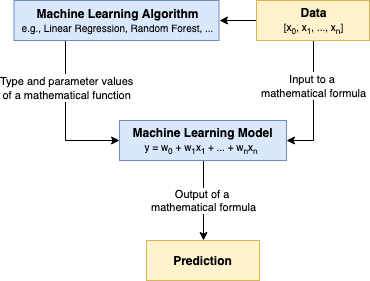
\includegraphics[width=\textwidth]{figures/drawio/machine-learning-model.png}
                \end{figure}
            \end{column}
        \end{columns}
    \end{frame}

    \subsection{Learning Styles}
    
    \begin{frame}{Learning Styles Overview}
        \begin{figure}
            \label{fig:learning-styles}
            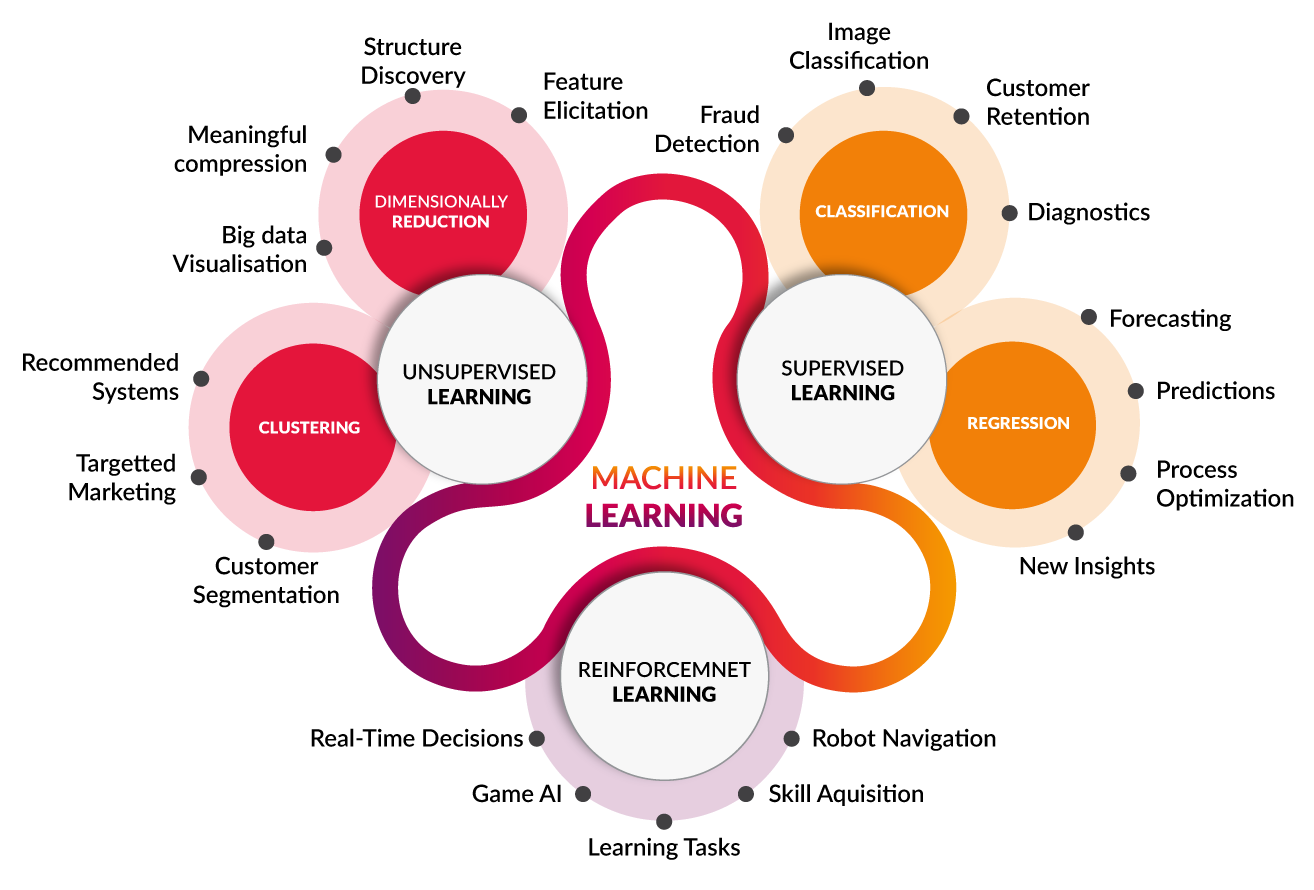
\includegraphics[width=.7\textwidth]{figures/external/learning-styles.png}
        \end{figure}
    \end{frame}

    \begin{frame}{Supervised Learning}
        \begin{columns}
            \begin{column}{.6\textwidth}
                \begin{itemize}
                    \item \textbf{Supervised learning} refers to a group of algorithms that require a \textbf{dataset of exemplary input-output combinations}. Those input-output combinations consist of \textbf{features} used to make predictions and an expected outcome called \textbf{label}.
                    \item During the learning process the \textbf{feature sets are iteratively fed to the algorithm} and for each set the it uses the \textbf{current state of model parameters} and returns a \textbf{prediction}.
                    \item The \textbf{prediction error} is a \textbf{feedback for the algorithm} of \textbf{what went wrong and how to update the model parameters} in order to \textbf{decrease the error in future predictions}. 
                    \item The major goal is to find \textbf{parameter values} that will allow a model to \textbf{perform well on historical data} and to \textbf{make predictions on unknown data} that have been part of the training dataset.
                \end{itemize}
            \end{column}
            \begin{column}{.4\textwidth}
                \begin{figure}
                    \label{fig:supervised-learning}
                    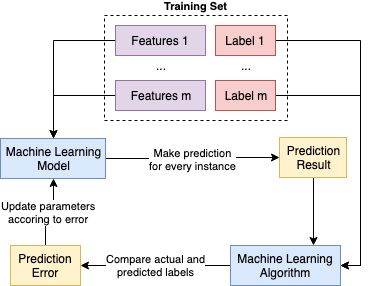
\includegraphics[width=\textwidth]{figures/drawio/supervised-learning.png}
                \end{figure}
            \end{column}
        \end{columns}
    \end{frame}

    \begin{frame}{Unsupervised Learning}
        \begin{columns}
            \begin{column}{.6\textwidth}
                \begin{itemize}
                    \item There are of course datasets whose \textbf{feature have no reference to known or labeled outcomes} and so there is no chance for a supervised learning algorithm to work.
                    \item For this cases, \textbf{unsupervised learning} kicks in which refers to a group of algorithms that try to \textbf{draw inference from non-labeled datasets}.
                    \item As there are no known outcomes, unsupervised learning can \textbf{not give correct answers} but rather the results must be \textbf{individually interpreted by a human} which in turn requires \textbf{domain knowledge and business expertise}.
                    \item Models based on this group of algorithms are mainly used for \textbf{discovering unknown patterns or structures} that are \textbf{hidden in the data} or to \textbf{reduce the dimensionality} of data by compressing features into \textbf{principal values} which conveys \textbf{similar information} concisely.
                \end{itemize}
            \end{column}
            \begin{column}{.4\textwidth}
                \begin{figure}
                    \label{fig:unsupervised-learning}
                    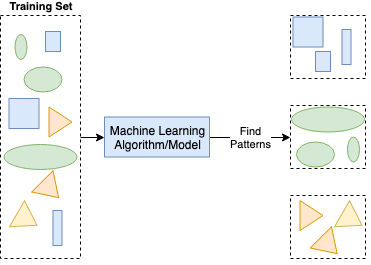
\includegraphics[width=\textwidth]{figures/drawio/unsupervised-learning.png}
                \end{figure}
            \end{column}
        \end{columns}
    \end{frame}

    \begin{frame}{Reinforcement Learning}
        \begin{columns}
            \begin{column}{.6\textwidth}
                \begin{itemize}
                    \item Algorithms from the group of \textbf{reinforcement learning} produce \textbf{agents} rather than classical models that \textbf{receive information from the environment and react to it} by performing an \textbf{action}.
                    \item The information the agent receives from the environment in form of \textbf{numerical data} is called \textbf{state} which is stored and then used for choosing the right action.
                    \item As a result of the action, the agent receives a \textbf{reward} that can be either \textbf{positive or negative} which is then used as a \textbf{feedback} to the agent in order to \textbf{update its parameters} and \textbf{change its future actions}.
                    \item The process of learning and training is a process of \textbf{trial and error}. The agents finds itself in \textbf{various states} and gets\textbf{ punished every time it takes the wrong action} and thus \textbf{starts learning how to take better actions}.
                \end{itemize}
            \end{column}
            \begin{column}{.4\textwidth}
                \begin{figure}
                    \label{fig:reinforcement-learning}
                    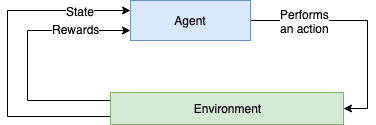
\includegraphics[width=\textwidth]{figures/drawio/reinforcement-learning.png}
                \end{figure}
            \end{column}
        \end{columns}
    \end{frame}

    \stepcounter{openexercise}
    \begin{frame}{Open Exercise \arabic{openexercise}}
        For each of the following cases below, state whether a supervised or an unsupervised learning algorithm would best address the particular problem.
        \begin{enumerate}[a)]
            \item Predicting the next day's return of a particular stock based on the close prices over the last 10 years of the corresponding stock.
            \item Grouping patients suffering from heart disease into different clusters based on a dataset with medical records with the objective of tailoring individual treatments for such patients.
            \item Classifying whether the content of an e-mail should be considered as spam or as regular correspondence.
        \end{enumerate}
    \end{frame}

    \subsection{Learning Tasks}
    
    \begin{frame}{Learning Tasks Overview}
        \begin{figure}
            \label{fig:learning-tasks}
            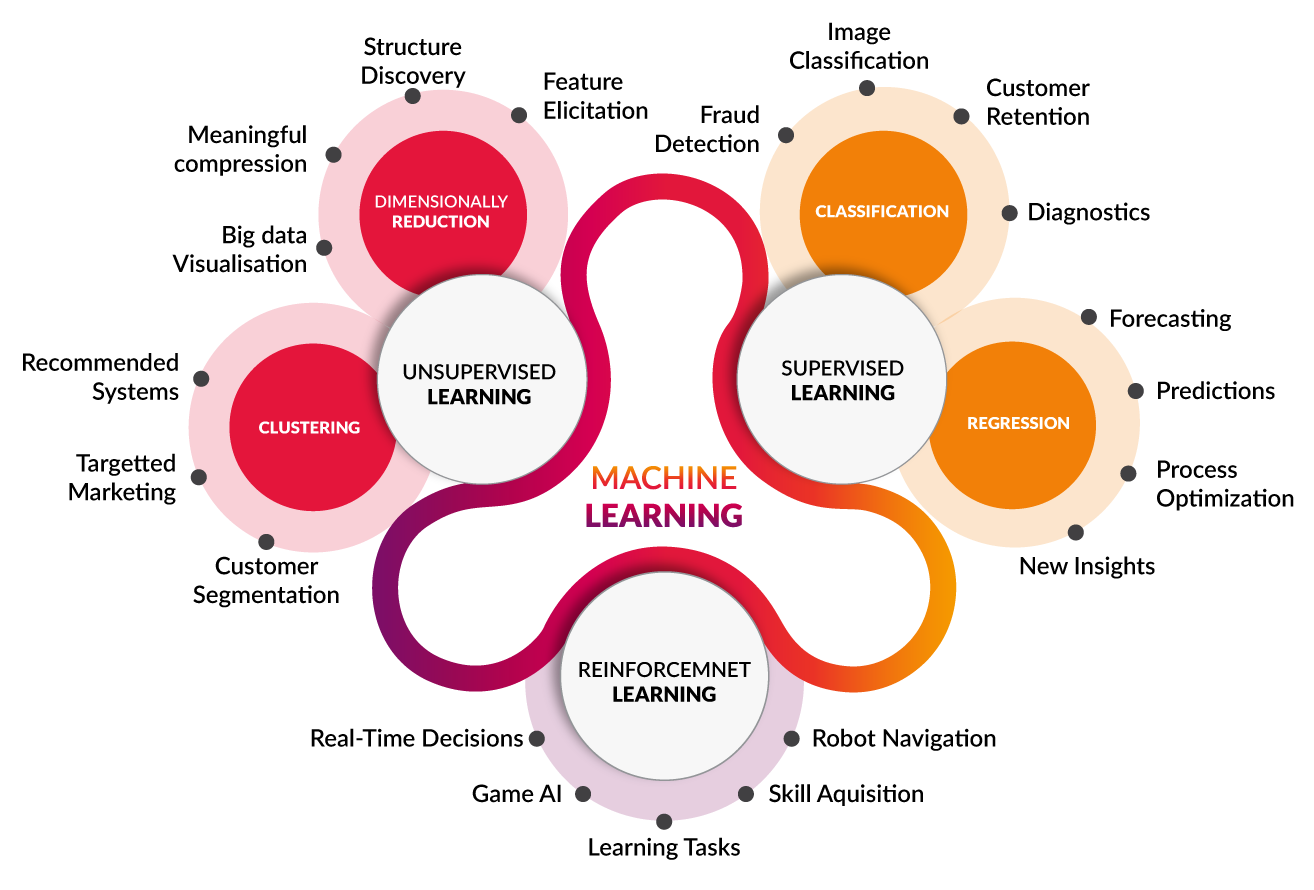
\includegraphics[width=.7\textwidth]{figures/external/learning-styles.png}
        \end{figure}
    \end{frame}

    \begin{frame}{Regression}
        \begin{columns}
            \begin{column}{.6\textwidth}
                \begin{itemize}
                    \item \textbf{Regression} is the process of \textbf{modeling and predicting a continuous, numerical outcome} that are often \textbf{quantities}, such as amounts and sizes.
                    \item Some algorithms have the word regression in their name, such as linear regression and logistic regression, which can make things confusing because \textbf{linear regression is a regression} algorithm whereas \textbf{logistic regression is a classification algorithm}. 
                    \item Examples include \textbf{predicting real-estate prices, stock price movements, or student test scores}.
                \end{itemize}
            \end{column}
            \begin{column}{.4\textwidth}
                \begin{figure}
                    \label{fig:regression-task}
                    \includegraphics[width=0.8\textwidth, keepaspectratio]{figures/regression-task.pdf}
                \end{figure}
            \end{column}
        \end{columns}
    \end{frame}

    \begin{frame}{Classification}
        \begin{columns}
            \begin{column}{.6\textwidth}
                \begin{itemize}
                    \item \textbf{Classification} is the process of \textbf{modeling and predicting a discrete class label} that is often not measurable but observable.
                    \item When there are only two classes to predict, usually 1 or 0 values, then it is called \textbf{binary classification} and when there are more than two class labels to predict it is called \textbf{multi-classification}.
                    \item Examples include predicting \textbf{employee churn, email spam, financial fraud, and student letter grades}.
                \end{itemize}
            \end{column}
            \begin{column}{.4\textwidth}
                \begin{figure}
                    \label{fig:classification-task}
                    \includegraphics[width=0.8\textwidth, keepaspectratio]{figures/classification-task.pdf}
                \end{figure}
            \end{column}
        \end{columns}
    \end{frame}

    \begin{frame}{Clustering}
        \begin{columns}
            \begin{column}{.6\textwidth}
                \begin{itemize}
                    \item Clustering is an \textbf{unsupervised learning} task for finding \textbf{natural groupings of observations} (i.e. clusters) based on the \textbf{inherent structure within a dataset}. 
                    \item Because clustering is unsupervised (there is no right answer), \textbf{data visualization is usually used to evaluate results}. If there is a right answer (i.e. you have pre-labeled clusters in your training set), then classification is typically more appropriate.
                    \item Examples include \textbf{customer segmentation, grouping similar items in e-commerce, and social network analysis}.
                \end{itemize}
            \end{column}
            \begin{column}{.4\textwidth}
                \begin{figure}
                    \label{fig:clustering-task}
                    \includegraphics[width=0.8\textwidth, keepaspectratio]{figures/clustering-task.pdf}
                \end{figure}
            \end{column}
        \end{columns}
    \end{frame}

    \begin{frame}{Dimensionality Reduction}
        \begin{columns}
            \begin{column}{.6\textwidth}
                \begin{itemize}
                    \item As learning problems often involve \textbf{several hundreds of features} for each training instance, training can get \textbf{extremely slow} and the model tends to \textbf{learn the noise} in the data.
                    \item Therefore, dimensionality reduction as an \textbf{unsupervised learning} task aims to \textbf{reduce the complexity of large datasets} while simultaneously keeping the \textbf{loss of information} at a minimum.  
                    \item However, every dimensionality reduction is accompanied by a loss of information. Therefore it is important to trade off \textbf{understandability and processibility} for the \textbf{amount of information content}.
                    \item Dimensionality reduction not only \textbf{fastens the time required for computing} by removing redundant features but also allows to \textbf{visualize multi-dimensional data precisely}.
                \end{itemize}
            \end{column}
            \begin{column}{.4\textwidth}
                \begin{figure}
                    \label{fig:dimensionality-reduction-task}
                    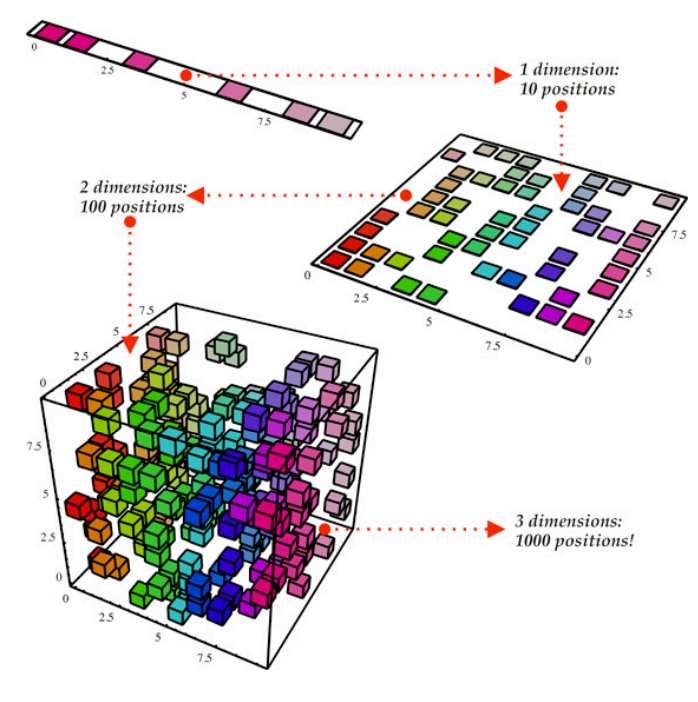
\includegraphics[width=.8\textwidth, cframe=gray]{figures/external/dimensionality-reduction.png}
                \end{figure}
            \end{column}
        \end{columns}
    \end{frame}

    \begin{frame}{Anomaly Detection}
        \begin{columns}
            \begin{column}{.6\textwidth}
                \begin{itemize}
                    \item In complex businesses, \textbf{several hundreds of metrics and dimensions} exist which makes it \textbf{impossible to track them all manually}. Reducing the amount of metrics or dimensions may \textbf{prevent to track and analyze all relevant business aspects}.
                    \item Therefore, anomaly detection is an (mostly) \textbf{unsupervised learning} task for \textbf{identifying unusual patterns} - preferably in real-time - that do not conform to \textbf{expected behavior}.
                    \item Examples include \textbf{intrusion detection, system health monitoring, performance tracking, and fraud detection}.
                \end{itemize}
            \end{column}
            \begin{column}{.4\textwidth}
                \begin{figure}
                    \label{fig:anomaly-detection-task}
                    \includegraphics[width=0.8\textwidth, keepaspectratio]{figures/anomaly-detection-task.pdf}
                \end{figure}
            \end{column}
        \end{columns}
    \end{frame}

    \stepcounter{openexercise}
    \begin{frame}{Open Exercise \arabic{openexercise}}
        For each of the following cases below, state whether you would treat the problem as a classification or a regression task.

        \begin{enumerate}[a)]
            \item Predicting whether a company will declare bankruptcy within the next month by using data of similar companies that had previously been at risk of bankruptcy.
            \item Predicting the tomorrow's temperature (in degree Centigrade) by using meteorological observations (e.g., temperature, air pressure) over the past 20 years.
        \end{enumerate}
    \end{frame}	
\end{document}